\documentclass[ a4paper]{article}

\usepackage[T2A]{fontenc}
\usepackage[utf8]{inputenc}
\usepackage[russian]{babel}

\usepackage{csvsimple}%   чтение  csv файлов 


\usepackage[unicode, colorlinks, linkcolor=blue, citecolor=blue]{hyperref}
\usepackage{amsmath}
\usepackage{graphicx}
\graphicspath{{pictures/}}
\DeclareGraphicsExtensions{.pdf,.png,.jpg}

\usepackage[]{geometry}
\geometry
{
	a4paper,
	total={170mm,257mm},
	left=25mm,
	top=19mm,
	right=25mm
}

\begin{document}
	\selectlanguage{russian}
	%----------------------------------Шапка--------------------------------------
	\begin{figure}[htb]
		\begin{minipage}[c]{0.12\textwidth}
			
\includegraphics[scale=0.25]{AU}
		\end{minipage}
		\hfill
		\begin{minipage}[t]{0.9\textwidth}
			{\Large\bfseries Санкт-Петербургский национальный исследовательский Академический университет имени Ж.И.~Алфёрова\\Российской академии наук}
		\end{minipage}
		\rule{164mm}{0.3mm}
	\end{figure}
	
	\begin{center}
		{\large\textbf{Рабочий протокол и отчёт по лабораторной работе №4 }}\\
		Свиридов Фёдор, Александр Слободнюк, Владимир Попов
	\end{center}
	\begin{center}
		\Large\bfseries{<<Свободные затухающие колебания в параллельном LC-контуре>>}\\
	\end{center}
	%-------------------------------------------------------------------------------
	{\parindent=0pt\textbf{Исходные данные.}}\\
	\begin{equation}
		U(t)=U_me^{-\beta t}\sin(\omega t + \alpha)
			\end{equation}
				\begin{equation}
			T=2\pi\sqrt{LC}
		\end{equation}
		\begin{equation}
			\beta = \frac{R}{2L}
		\end{equation}
			\begin{equation}
		\omega=\sqrt{\omega_0^2-\beta^2}
	\end{equation}
		\begin{equation}
	\lambda=\frac{U(t)}{U(t+T)}=\beta T
\end{equation}
		\begin{equation}
	Q\approx\frac{1}{R}\,\sqrt{\frac{L}{C}}
\end{equation}
	{\parindent=0pt\textbf{Результаты прямых измерений.}}\\
\begin{figure}[htb]
	\begin{minipage}[c][4.3in][t]{0.2\textwidth}
		\centering Контур №1\\
		L = 5,7 мГн\\
		 C = 97,9 нФ\\
		  R = 16,65 Ом\\
		  time/div = 0,1 мс\\
		  volts/div = 0,1 B\\
		  \vspace{0.25cm}
		\csvreader[tabular=c|r, table head=\hline $t${,} div & $U${,} div\\\hline]
		{1.csv}{X=\X,Y=\Y}
		{  \X & \Y}
	\end{minipage}
	\hfill
	\begin{minipage}[c][4.3in][t]{0.2\textwidth}
				\centering Контур №2\\
		L = 5,7 мГн\\
		C = 97,9 нФ\\
		R = 5,3 Ом\\
		time/div = 0,1 мс\\
		volts/div = 0,1 B\\
		\vspace{0.25cm}
	\csvreader[tabular=c|r, table head=\hline $t${,} div & $U${,} div\\\hline]
	{2.csv}{X=\X,Y=\Y}
	{  \X & \Y}
	\end{minipage}
\hfill
			\begin{minipage}[c][4.3in][t]{0.2\textwidth}
						\centering Контур №3\\
				L = 5,7 мГн\\
				C = 1 мкФ\\
				R = 5,3 Ом\\
				time/div = 0,5 мс\\
				volts/div = 0,1 B\\
				\vspace{0.25cm}
	\csvreader[tabular=c|r, table head=\hline $t${,} div & $U${,} div\\\hline]
	{3.csv}{X=\X,Y=\Y}
	{  \X & \Y}
\end{minipage}
\hfill
\begin{minipage}[c][4.3in][t]{0.2\textwidth}
							\centering Контур №4\\
	L = 5,7 мГн\\
	C = 1 мкФ\\
	R = 16,65 Ом\\
	time/div = 0,5 мс\\
	volts/div = 0,1 B\\
	\vspace{0.25cm}
	\csvreader[tabular=c|r, table head=\hline $t${,} div & $U${,} div\\\hline]
	{4.csv}{X=\X,Y=\Y}
	{  \X & \Y}
\end{minipage}
\rule{164mm}{0.3mm}
\end{figure}

{\parindent=0pt\textbf{Обработка результатов и расчёт косвенных величин.}}\\
{\parindent=0pt
$\bullet$ Период колебаний $T$\\
Для 1-го и 2-го контура по формуле (2)  $T_{12}  = 0,158$ мс. Из опыта $T_{12}=0,155$ мс\\
Для 3-го и 4-го контура по формуле (2)  $T_{34}  = 0,474$ мс. Из опыта $T_{34}=0,506$ мс\\

$\bullet$ Коэффициент затухания $\beta$ \\
$\beta_1=1461\;c^{-1}$\\
$\beta_2=465\;c^{-1}$\\
$\beta_3=465\;c^{-1}$\\
$\beta_4=1461\;c^{-1}$\\

$\bullet$ Логарифмический декремент $\lambda$\\
$\lambda_1=0,226$\\
$\lambda_2=0,074$\\
$\lambda_3=0,235$\\
$\lambda_4=0,730$\\

$\bullet$ Время затухания $\tau=\frac{1}{\beta}$\\
$\tau_1=0,684\;\mbox{мc}$\\
$\tau_2=2,150\;\mbox{мc}$\\
$\tau_3=2,150\;\mbox{мc}$\\
$\tau_4=0,684\;\mbox{мc}$\\

$\bullet$ Добротность $Q$\\
$Q_1=14,49$\\
$Q_2=45,53$\\
$Q_3=14,24$\\
$Q_4=4,53$\\
}
\begin{center}
		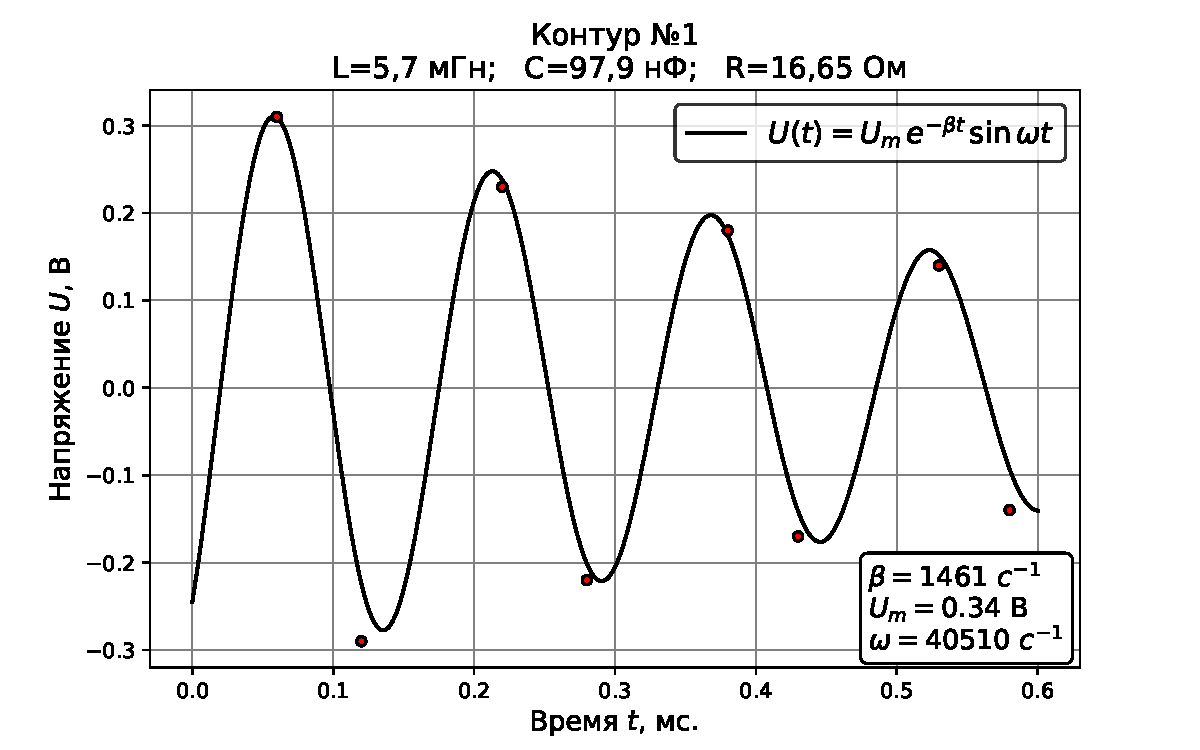
\includegraphics[scale=0.7]{1.pdf}
\end{center}

\begin{center}
	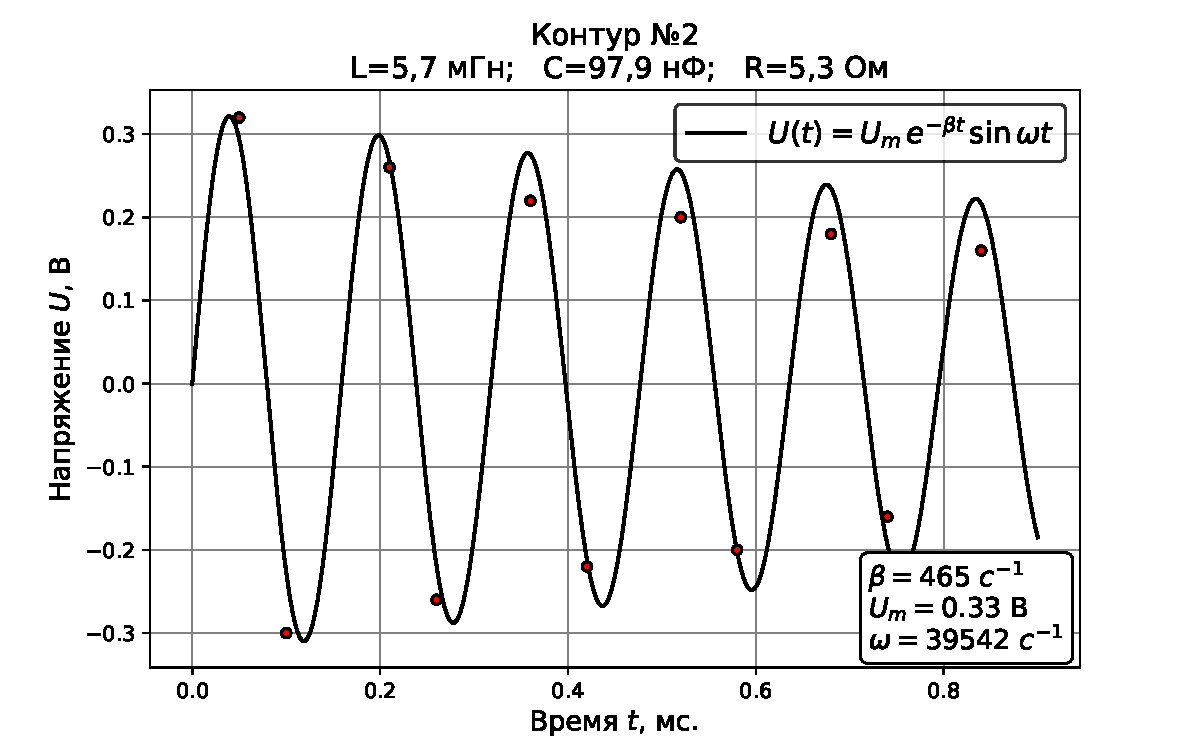
\includegraphics[scale=0.7]{2.pdf}
\end{center}

\begin{center}
	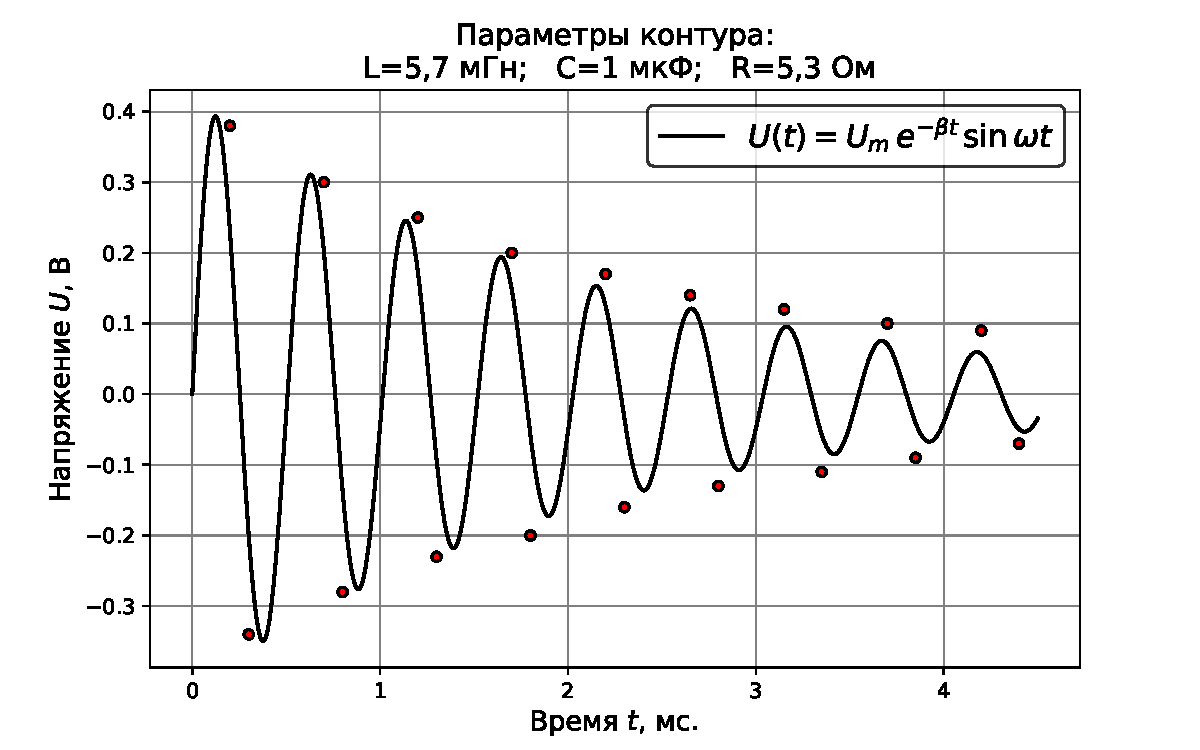
\includegraphics[scale=0.7]{3.pdf}
\end{center}

\begin{center}
	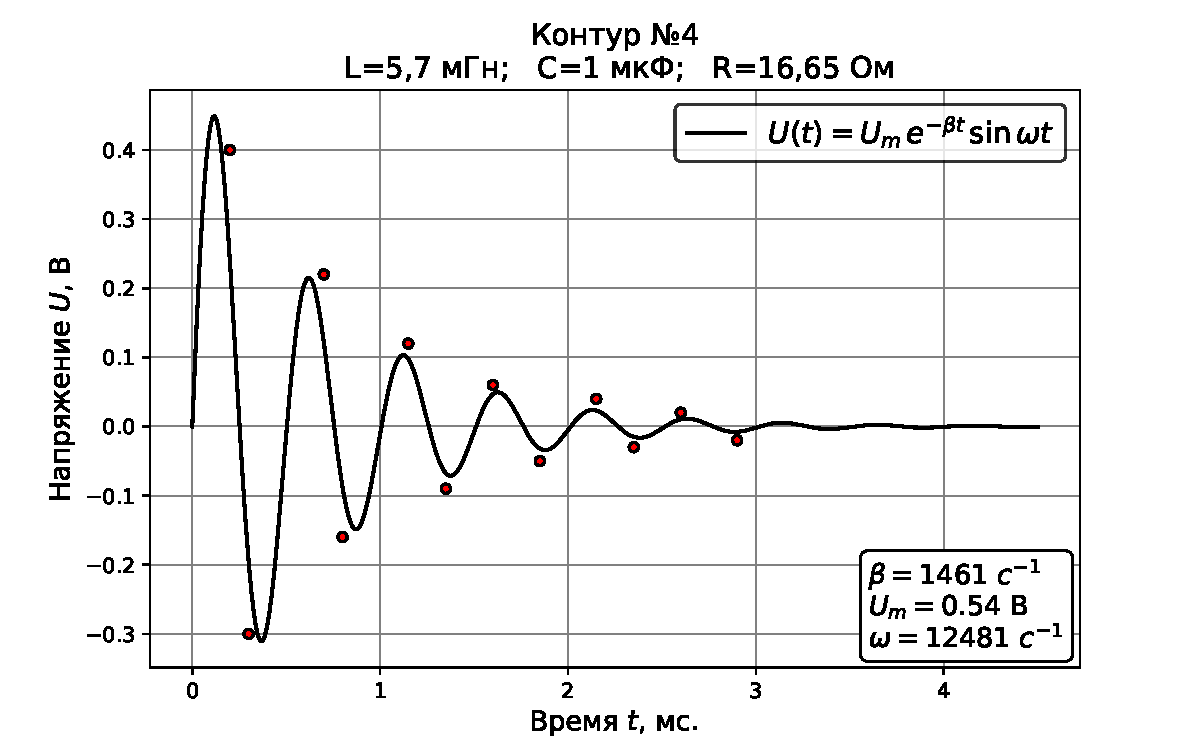
\includegraphics[scale=0.7]{4.pdf}
\end{center}

{\parindent=0pt\textbf{Выводы.}}\\
Мы провели измерения свободных затухающих колебаний напряжения в LC-контурах с разными параметрами. 
На основе полученных данных были найдены следующие величины: период колебаний~$T$, коэффициент затухания $\beta$, 
логарифмический декремент $\lambda$, время затухания $\tau$, добротность~$Q$.

В опыте было обнаружено необычное  поведение затухающих колебаний: их полупериоды (время, за которое заряды на обкладках конденсатора меняют знак) 
не равны, что противоречит уравнению колебаний $U(t)=U_me^{-\beta t}\sin(\omega t + \alpha)$, так как данная функция обладает симметрией. 
Приведём значения полупериодов всех 4-ёх контуров:
\begin{center}
	\begin{tabular}{|c|c|c|c|c|c|c|c|c|c|c|c|c|c|c|c|}
		\hline
		$hT_1$, div&  0.6& 1 & 0.6& 1 & 0.5& 1 & 0.5& & & & & & && \\
		\hline
		$hT_2$, div&  0.5& 1.1& 0.5& 1.0 & 0.6& 1 & 0.6& 1 & 0.6& 1 & & & && \\
		\hline
		$hT_3$, div& 0.2& 0.8& 0.2& 0.8& 0.2& 0.8& 0.2& 0.8& 0.2& 0.7& 0.3& 0.7& 0.4& 0.7& 0.3 \\
		\hline
		$hT_4$, div&0.2& 0.8& 0.2& 0.7& 0.4& 0.5& 0.5& 0.6& 0.4& 0.5& 0.6& & & &\\
		\hline
	\end{tabular}
\end{center}

Различия очень хорошо видны в 3 контуре:
\begin{center}
	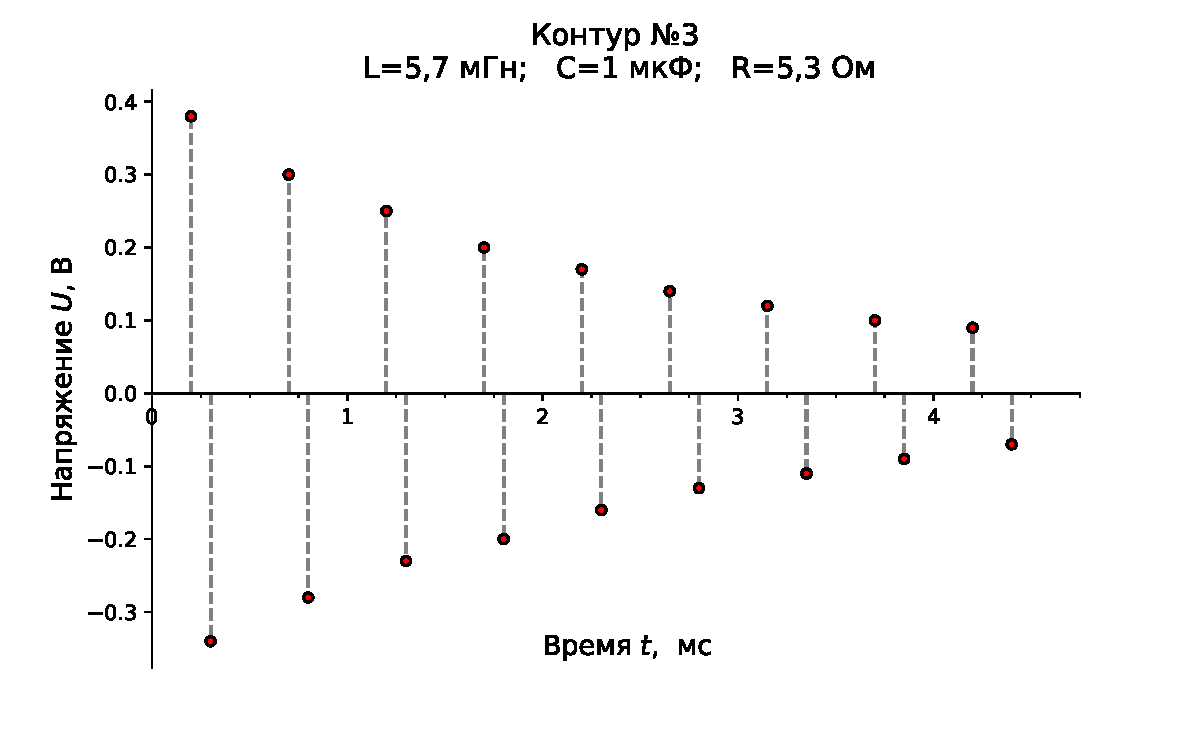
\includegraphics[scale=0.7]{pic.pdf}
	\end{center}
Таким образом, перетекание заряда в одном направление происходит быстрее чем в другом. 
Объяснения данному явлению мы не знаем, но можно предположить, что, так как период однозначно определяют L и C, то 
в осцилляторе либо  индуктивность, либо ёмкость конденсатора зависит от направления тока.
	\end{document}
